\section{IoT}
En esta seccion se demostrara como usar el Azure Sphere para conectarse al servicio Azure IoT Hub de Microsoft.
\subsection{Registro en Azure}
Registre una cuenta gratuita en \href{https://azure.microsoft.com/es-mx/free}{Azure}. Para esto,	 necesita obligatoriamente un numero telefónico y una tarjeta de crédito o débito para verificar su identidad.

Ahora se tiene que crear un IoT Hub, este es un servicio de la nube que funciona como un centro de comunicación entre distintos aplicaciones IoT. Para crearlo, en el panel de Azure, selecciona Create a resource.
\begin{figure}[h]
	\centering
	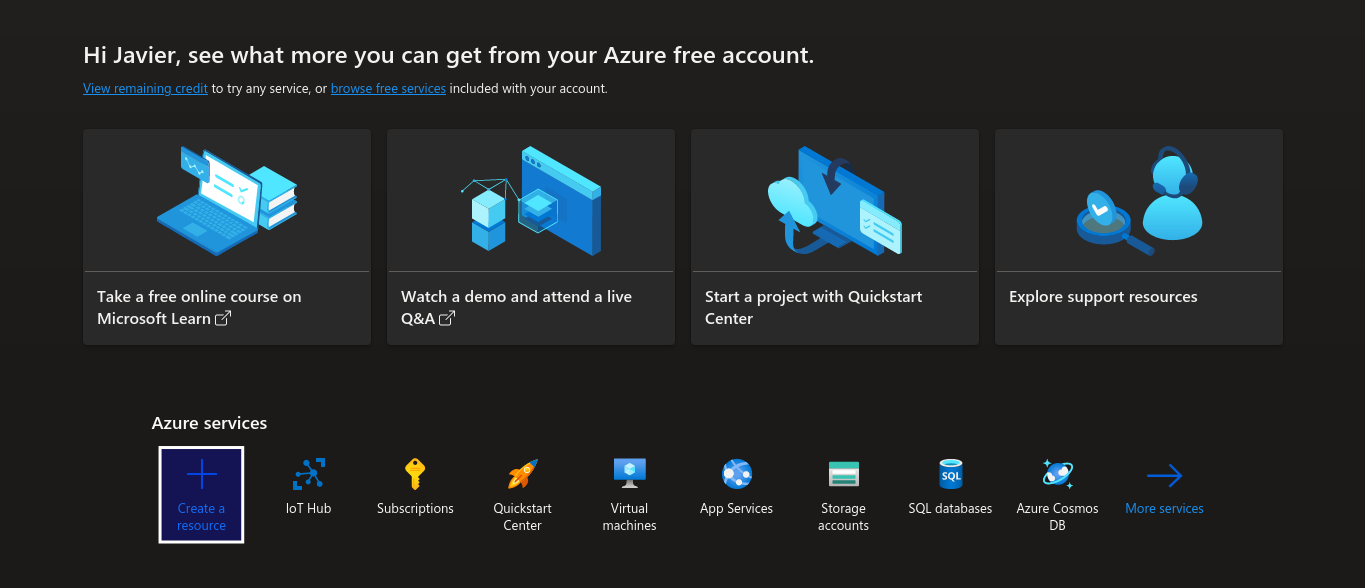
\includegraphics[width=0.75\textwidth,height=\textheight,keepaspectratio]{Azure1}
\end{figure}
En la pagina de Create a resource, en la sección de categorías, elige Internet of Things y presiona IoT Hub.
\begin{figure}[h]
	\centering
	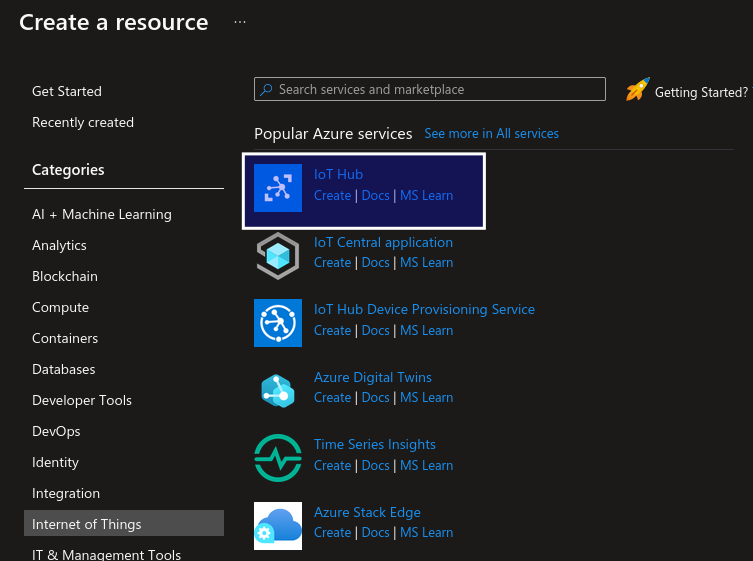
\includegraphics[width=0.75\textwidth,height=\textheight,keepaspectratio]{Azure2}
\end{figure}
Llena todos los datos para el registro de tu IoT Hub. El resource group lo puedes crear ahi mismo. La región elige la de tu preferencia. El nivel elige gratuito. El nombre del Hub solo tienen que ser letras. Al tener todo listo da click en review + create y para confirmar create.
\begin{figure}[h]
	\centering
	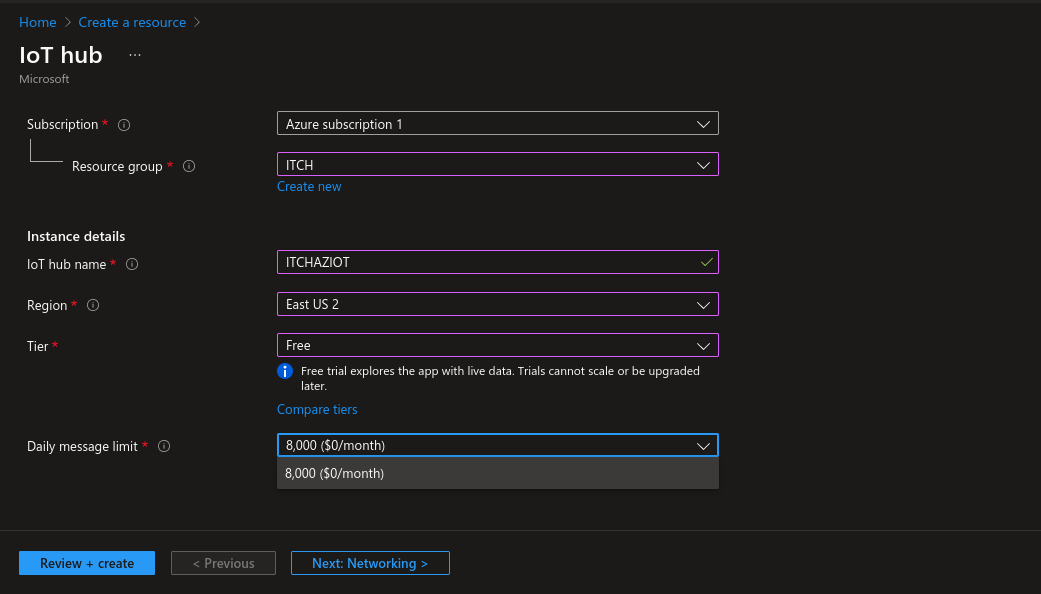
\includegraphics[width=0.75\textwidth,height=\textheight,keepaspectratio]{Azure3}
\end{figure}
\subsection{Certificado del Azure Sphere}
En la terminal, ejecutar el siguiente comando.
\begin{verbatim}
	azsphere ca-certificate download --destination CAcertificate.cer
\end{verbatim}
Esto generara un certificado en el directorio que se encuentre la terminal.
\subsection{Subir el certificado al Iot hub}
Navega al IoT hub que creaste.

\begin{figure}[h]
	\centering
	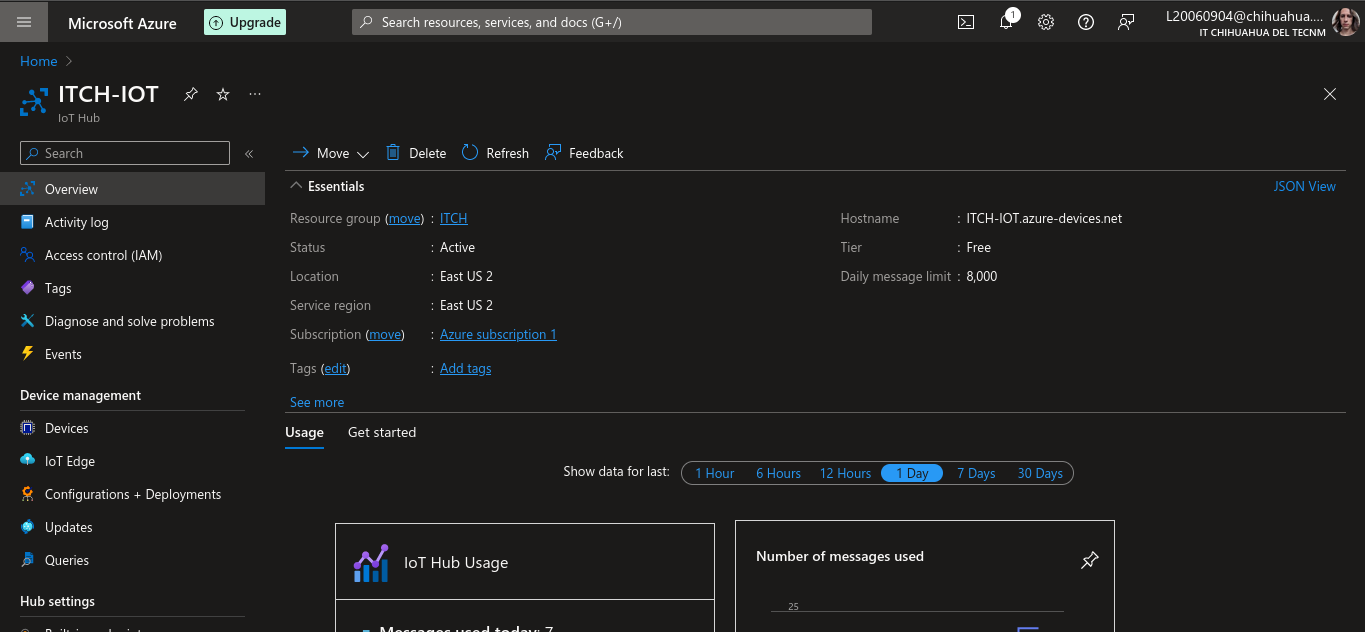
\includegraphics[width=0.75\textwidth,height=\textheight,keepaspectratio]{Azure4}
\end{figure}
\pagebreak
Ve a la sección de certificados.
\begin{figure}[h]
	\centering
	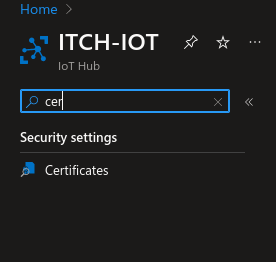
\includegraphics[width=0.75\textwidth,height=0.35\textheight,keepaspectratio]{Azure5}
\end{figure}

Ya estando en la sección, presiona el botón de add.
\begin{figure}[h]
	\centering
	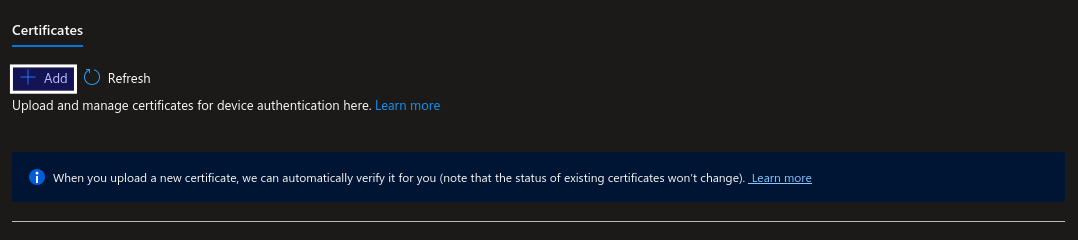
\includegraphics[width=0.9\textwidth,height=\textheight,keepaspectratio]{Azure6}
\end{figure}
\pagebreak

Agrega el nombre, el archivo del certificado y marca la casilla de "Set certificate status to verified on upload".
\begin{figure}[h]
	\centering
	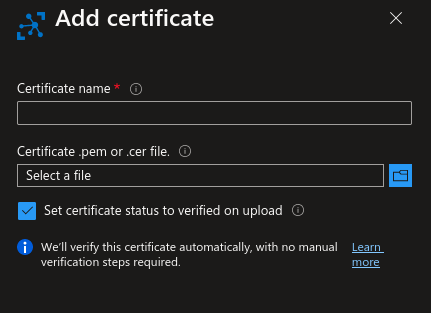
\includegraphics[width=0.9\textwidth,height=\textheight,keepaspectratio]{Azure7}
\end{figure}
\subsection{Agregar dispositivo}
En la pagina del IoT Hub, navega a la sección de dispositivos.
\begin{figure}[h]
	\centering
	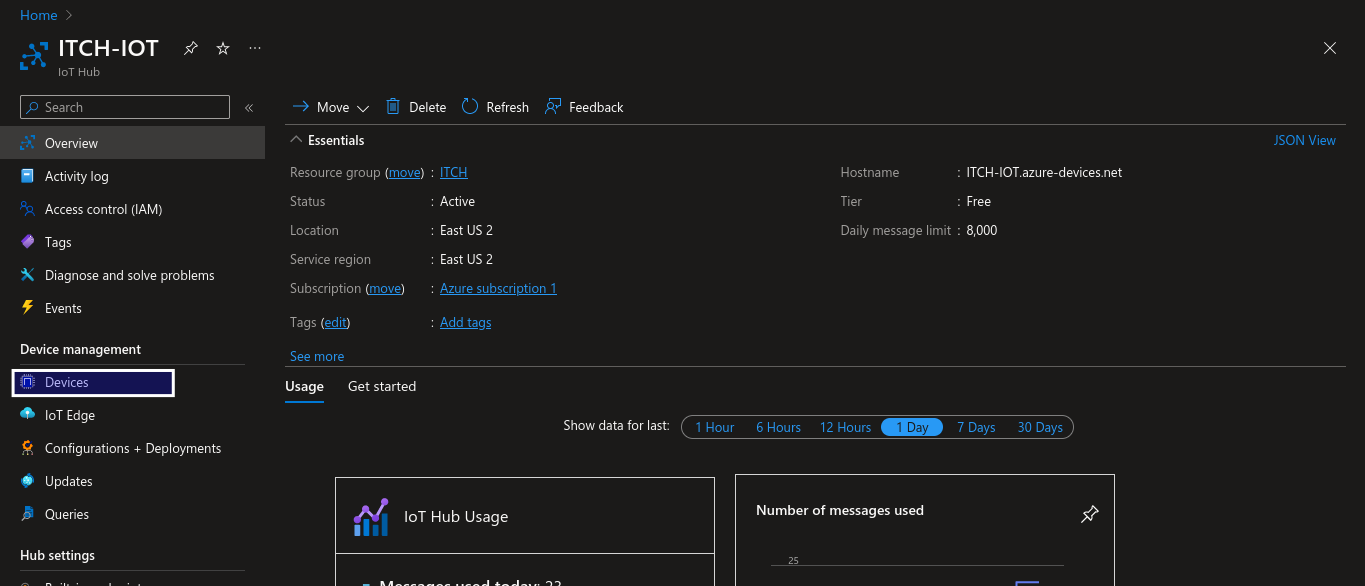
\includegraphics[width=0.75\textwidth,height=\textheight,keepaspectratio]{Azure8}
\end{figure}

Estando en la sección, presiona el botón de add device
\begin{figure}[h]
	\centering
	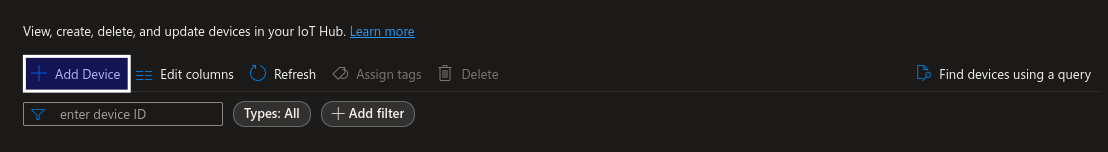
\includegraphics[width=0.9\textwidth,height=\textheight,keepaspectratio]{Azure9}
\end{figure}
\pagebreak

Agrega el id del dispositivo, este lo obtienes en la terminal con el siguiente comando (El dispositivo debe estar conectado a la computadora):
\begin{verbatim}
	azsphere device show-attached
\end{verbatim}
En el tipo de autenticación eliges X.509 CA Signed. Despues presiona save.
\begin{figure}[h]
	\centering
	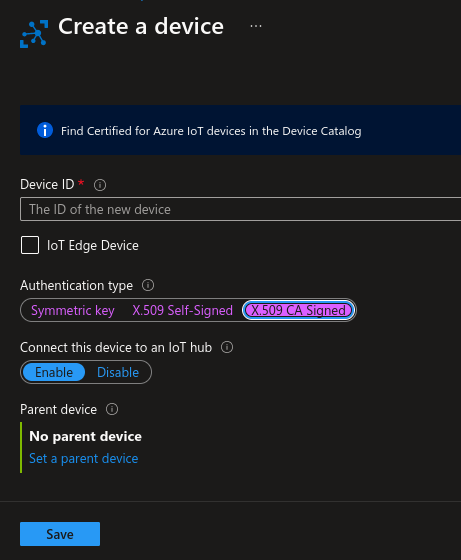
\includegraphics[width=0.9\textwidth,height=\textheight,keepaspectratio]{Azure10}
\end{figure}
